\documentclass{beamer}
\usetheme{Copenhagen}
\usepackage{float}
\beamertemplatenavigationsymbolsempty
\usepackage[font=footnotesize]{caption}
\captionsetup[figure]{labelformat=empty}

\usepackage[utf8]{inputenc}
\usepackage{framed}
\usepackage[super]{nth}

\usepackage{tabularx}
\usepackage{xspace}
\usepackage{multirow}% http://ctan.org/pkg/multirow
\usepackage{diagbox}
\usepackage{changepage}

\title{8 novembre 2018 - \insertframenumber/\inserttotalframenumber}
%\subtitle{Using Beamer}
%
%\begin{figure}[!htb]
%    \centering
%    \begin{minipage}{.5\textwidth}
%        \centering
%        \includegraphics[scale=0.05]{logo-ensta.png}
%    \end{minipage}%
%    \begin{minipage}{0.5\textwidth}
%        \centering
%        \includegraphics[scale=0.12]{logo-ens.jpg}
%    \end{minipage}
%\end{figure}
%
%{\vfill Martin BAUW\\\textit{under the supervision of} Thibault TORALBA}
%\end{center}
%
\author{TC2 Project}
%\institute{University of ShareLaTeX}
%\date{\today}

%\date{mercredi 6 septembre 2017}

\begin{document}

\begin{frame}
\begin{center}
{ M2 AIC\\\footnotesize TC2: Introduction to Optimization}
\vfill
{\large
\begin{framed}
Black-Box Optimization Benchmarking\\ with the COCO platform\\ - \\Multiobjective Optimizer adaptive IBEA ($\epsilon$-indicator) 
\end{framed}
}
\vfill
% \begin{figure}
% \centering
% \includegraphics[scale=0.25]{logo_upsaclay.jpg}
% \end{figure}

{\footnotesize \vfill \textit{Group 1:} Martin BAUW, Robin DURAZ, Jiaxin GAO,\\ Hao LIU, Luca VEYRON-FORRER}
\end{center}
\end{frame}

\begin{frame}
\tableofcontents
\end{frame}

\section{Introduction}
\begin{frame}
IBEA: Indicator-Based Evolutionary Algorithm
\begin{itemize}
\item optimization: find decision space vectors leading to objective space minima
\item multiobjective: the objective space is multidimensional
\item evolutionary: decision space candidates follows an natural selection-like evolution
\item indicator-based: binary quality indicators to compare two Pareto set approximations
\end{itemize}
\end{frame}


\section{The algorithm}
\subsection{Overview of IBEA}
\begin{frame}
\begin{columns}[T]
\begin{column}{.48\textwidth}
Successive steps of IBEA:
\begin{enumerate}
\item Initialization
\item Fitness assignment % scale each objective to [0,1], calculate Is then c then fitness values
\item Environmental selection % update fitness values thanks to F()
\item Termination
\item Mating selection
\item Variation
\end{enumerate}
\end{column}
\begin{column}{.48\textwidth}
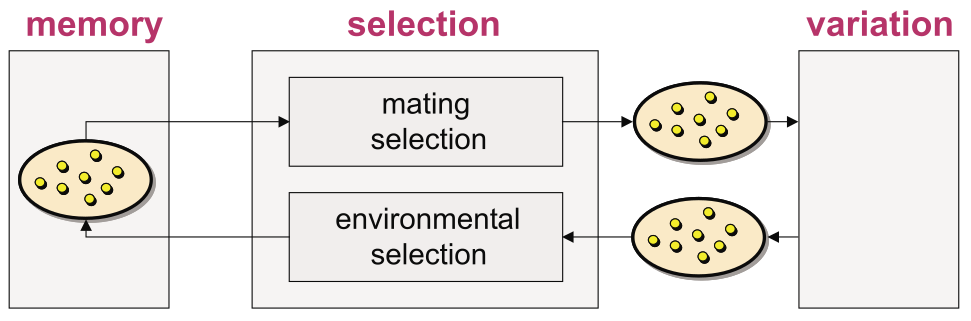
\includegraphics[scale=0.16]{stochasticSearchAlgorithm.png} \footnotemark
\end{column}
\end{columns}
\footnotetext[1]{Illustration from:\\ \textit{A Tutorial on Evolutionary Multiobjective
Optimization} - E. Zitzler, \\M. Laumanns, and S. Bleuler}
\end{frame}


\begin{frame}
\begin{adjustwidth}{-2.2em}{-2.2em}
\begin{itemize}
\item \underline{Binary quality indicators:}
\begin{equation}
I_{\epsilon^+ (A,B)} = min_{\epsilon} \{\forall x^2 \in B\ \exists x^1 \in A : f_i(x^1) - \epsilon \leq f_i (x^2)\ for\ i \in \{1,...,n\}\}
\end{equation}
\item \underline{Fitness values:}
\begin{equation}
F(x^1) = \sum_{x^2 \in P \backslash \{x^1\}} -e^{-\dfrac{I(\{x^1\},\{x^2\})}{ck}}
\end{equation}
\end{itemize}
\end{adjustwidth}
\begin{center}
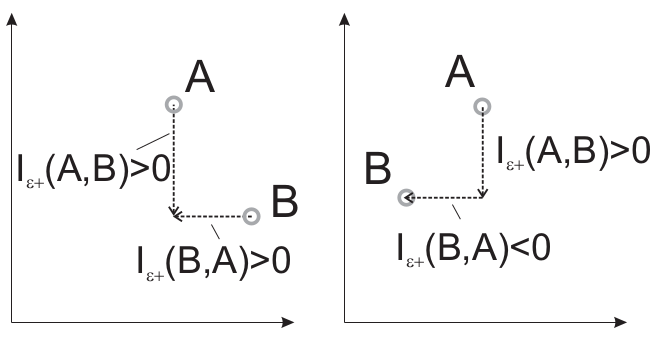
\includegraphics[scale=0.2]{binaryIndicators.png} \footnotemark
\end{center}
\footnotetext[1]{Illustration from:\\ \textit{Indicator-Based Selection in Multiobjective Search} - E. Zitzler and S. Künzli}
\end{frame}

\subsection{Selection and variation}
\begin{frame}
\frametitle{Recombination}
For recombination, we use a Simulated Binary Crossover (SBX) operator. A uniform probability pick in $[0,1]$ written $u$ determines the parameter used in computing the features (decision space coordinates) of the children.
\begin{itemize}
\item if the uniform probability pick $\leq 0.5$:
\begin{equation}
\beta_q = (2u)^{\frac{1}{\mu +1}}
\end{equation}
\item else:
\begin{equation}
\beta_q = (\frac{1}{2(1-u)})^{\frac{1}{\mu +1}}
\end{equation}
\end{itemize}
\end{frame}

\begin{frame}
\frametitle{Recombination}
Thus, we can compute the children's coordinates:

\begin{itemize}
\item first child:
\begin{equation}
child0[j] = 0.5((1+\beta_q)parent0[j]+(1-\beta_q)parent1[j])
\end{equation}
\item second child:
\begin{equation}
child1[j] = 0.5((1-\beta_q)parent0[j]+(1+\beta_q)parent1[j])
\end{equation}
\end{itemize}

\end{frame}

\begin{frame}
\frametitle{Mating selection and mutation}
Polynomial mutation operator:

The mutation operator modifies individuals by changing small parts in the associated vectors according to a given mutation rate.

\begin{itemize}
\item if the uniform probability pick $\leq 0.5$:
\begin{equation}
\sigma_L = (2u)^{\frac{1}{\mu +1}}-1 
\end{equation}
\begin{equation}
p_{mut}[j] = ind[j] + \sigma_L(ind[j]-Lo)
\end{equation}
\item else:
\begin{equation}
\sigma_R = (2(1-u))^{\frac{1}{\mu +1}} 
\end{equation}
\begin{equation}
p_{mut}[j] = ind[j] + \sigma_R(Up-ind[j])
\end{equation}
\end{itemize}

\end{frame}

\section{Our implementation}
\subsection{Code structure}
\begin{frame}

\end{frame}

\subsection{Improvements regarding the execution speed}
\begin{frame}

\end{frame}

\section{CPU timing and results}
\subsection{CPU timing and results}
\begin{frame}
  \frametitle{Computer specifications and batch options}
  \begin{itemize}
  \item Intel(R) Core(TM) i7-7500U CPU @ 2.70GHz
  \item Quad core CPU with 16GB RAM
  \end{itemize}
  \vspace{1em}
  Everything ran with a budget of 100\\
  \begin{itemize}
  \item Three batchs for dimensions 2, 3, 5, 10, 20
  \item First batch running alone, and two others together
  \item One batch for dimensions 40
  \end{itemize}
\end{frame}

\begin{frame}
  \frametitle{Options chosen to run the algorithm}
  \begin{itemize}
  \item Population size : 100
  \item Maximum number of generation : 100
  \item Scaling factor : 0.05
  \item Mutation rate : 0.01
  \item Recombination and mutation mu : 1
  \item Population initialization in range (-5, 5)
  \end{itemize}
\end{frame}

\begin{frame}
  %\frametitle{Time by function evaluation}
  \begin{table}[!htbp]
    \begin{tabular}{|p{3.8cm}|p{1.5cm}|p{1.5cm}|p{1.5cm}|}
      \hline
      \diagbox{Batch}{Dimension} & 2 & 3 & 5\\
      \hline
      Batch 1 on 3 & 6.0e-04 & 6.3e-04 & 8.1e-04\\
      \hline
      \multirow{2}{3.8cm}{Batch 2 and 3 on 3 run simultaneously} & 8.6e-04 & 8.6e-04 & 9.1e-04\\
      \cline{2-4}
                                 & 8.3e-04 & 8.4e-04 & 8.9e-04\\
      \hline
    \end{tabular}
    \begin{tabular}{|p{3.8cm}|p{2.47cm}|p{2.47cm}|}
      \hline
      \diagbox{Batch}{Dimension} & 10 & 20\\
      \hline
      Batch 1 on 3 & 8.3e-04 & 1.1e-03\\
      \hline
      \multirow{2}{3.8cm}{Batch 2 and 3 on 3 run simultaneously} & 1.1e-03 & 1.3e-03\\
      \cline{2-3}
                                 & 1.0e-03 & 1.3e-03\\
      \hline
    \end{tabular}
    \begin{tabular}{|p{3.8cm}|p{5.37cm}|}
      \hline
      \diagbox{Batch}{Dimension} & 40\\
      \hline
      Whole test suite & 4.2e-03\\
      \hline
    \end{tabular}
  \end{table}
\end{frame}


\begin{frame}
  \frametitle{Results}
  \begin{figure}
    \centering
    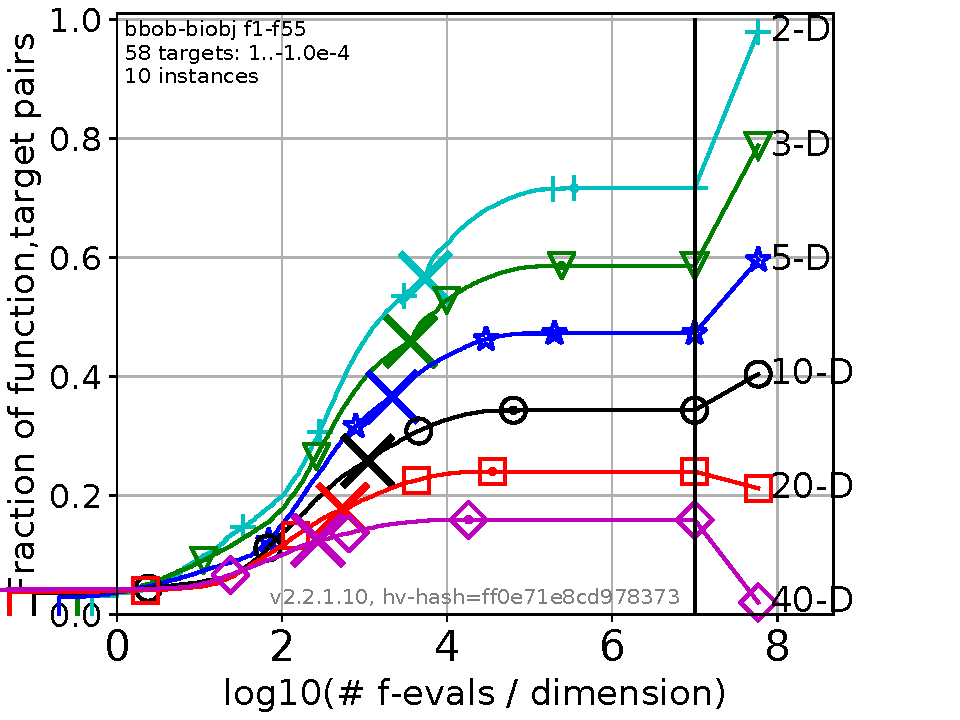
\includegraphics[scale=0.5]{pprldmany}
  \end{figure}
\end{frame}

\begin{frame}
  \frametitle{Results analysis}
  \begin{itemize}
  \item Comparatively better in higher dimensions
  \item Results globally good for an EMOA
  \end{itemize}
  \begin{itemize}
  \item More budget could have given better results
  \item A better initialization of population could lead to a sharper increase
    at the beginning
  \end{itemize}
\end{frame}

\subsection{Comparision with NSGA 2 and Random Search}
\begin{frame}
\frametitle{NSGA 2}

\end{frame}

\begin{frame}
\frametitle{Random Search}

\end{frame}

\section{Conclusion}
\begin{frame}
In our experiments, we majorly focused on the
comparison with NSGA-II and Random search:
\vskip 0.1in
IBEA VS Random search: IBEA outperformed Random search, a relatively good Pareto set approximation was given by IBEA.
 
IBEA VS NSGA-II: IBEA performed worse than NSGA-II.
\vskip 0.1in
Choosing a representation of the problem
addressed, an initial population, a method of selection, a crossover operator,
mutation operator, the probabilities of crossover and mutation, and the
insertion method creates a variant of MOEAs algorithms. 
\end{frame}

\section{Bibliography}
\begin{frame}
\frametitle{Non-exhaustive bibliography}
\begin{itemize}
\item \textit{Indicator-Based Selection in Multiobjective Search} - Zitzler, E. and Künzli, S.
\item \textit{A Tutorial on Evolutionary Multiobjective Optimization} - Zitzler, E. and Laumanns, M. and Bleuler, S.
\item \textit{Biobjective Performance Assessment with the {COCO} Platform} - Brockhoff, D. and Tu{\v s}ar, T. and Tu{\v s}ar, D. and Wagner, T. and Hansen, N. and Auger, A.
\end{itemize}
\end{frame}

\end{document}